\chapter{Deneysel Sonuçlar}
Sistemin 2 farklı güzergah üzerinde test edilmiştir. İlk güzergah Tablo 7.1'deki gibidir.

\begin{table}[!h]
\centering
\caption{1. Test güzergahı}
\label{my-label}
\begin{tabular}{|l|l|l|}
\hline
\textbf{Başlangıç}            & \textbf{Ulaşım Türü} & \textbf{Bitiş}                \\ \hline
Yenikapı Marmaray İstasyonu   & Yürüme               & Yenikapı Metro İstasyonu      \\ \hline
Yenikapı  Metro İstasyonu     & Haifa Raylı          & Zeytinburnu  Metro İstasyonu  \\ \hline
Zeytinburnu Metro İstasyonu   & Yürüme               & Zeytinburnu Tramvay İstasyonu \\ \hline
Zeytinburnu Tramvay İstasyonu & Tramvay              & Cevizlibağ Tramvay İstasyonu  \\ \hline
Zeytinburnu Tramvay İstasyonu & Yürüme               & Cevizlibağ Taksi Durağı       \\ \hline
Cevizlibağ Taksi Durağı       & Araba                & Esenler Metrosu               \\ \hline
\end{tabular}
\end{table}

\begin{figure}[!htbp]
\centering
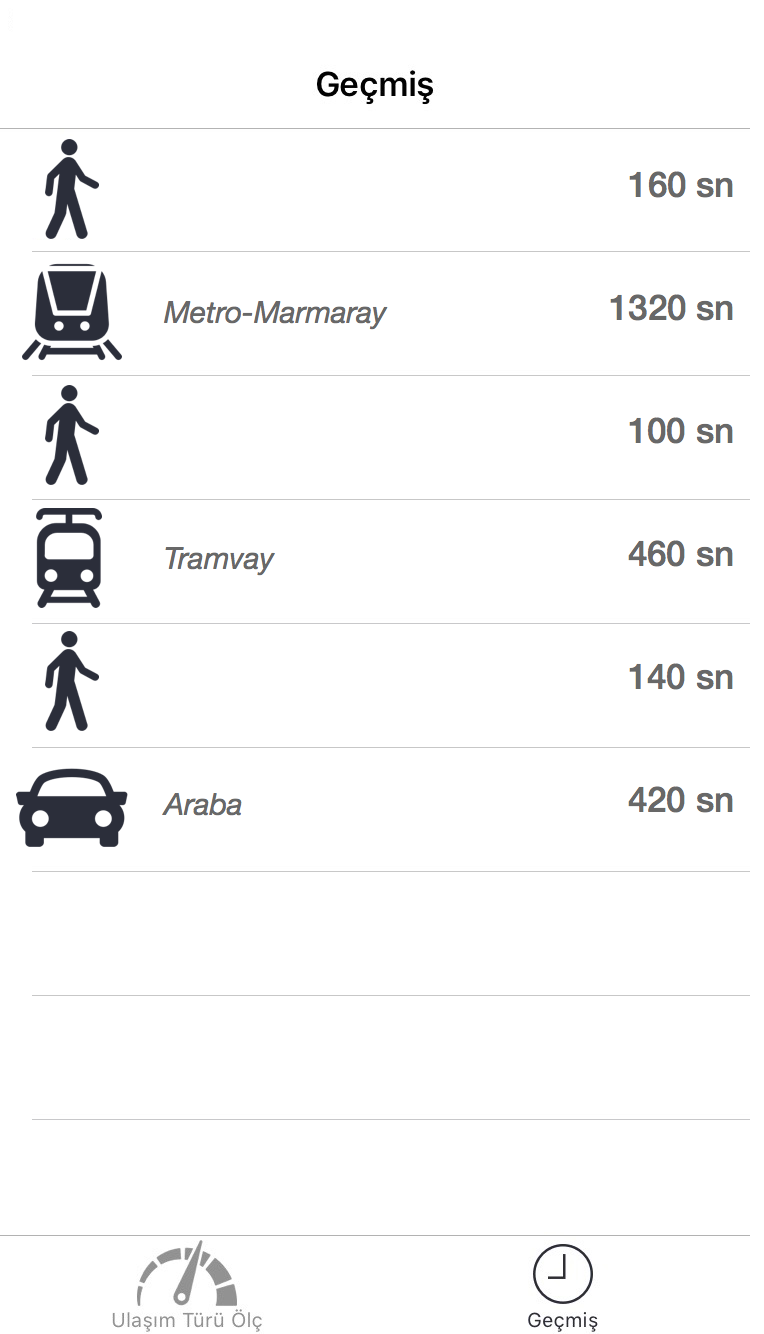
\includegraphics[scale=0.2]{projectChapters/images/rota_2.png}
\caption{1. güzergaha ait uygulama ekran çıktısı}
\end{figure}

\begin{table}[!h]
\centering
\caption{2. Test güzergahı}
\label{my-label}
\begin{tabular}{|l|l|l|}
\hline
\textbf{Başlangıç}          & \textbf{Ulaşım Türü} & \textbf{Bitiş}              \\ \hline
FSM Öğrenci Yurdu           & Yürüme               & YTÜ Davutpaşa Otobüs Durağı \\ \hline
YTÜ Davutpaşa Otobüs Durağı & Otobüs               & Cevizlibağ Otobüs Durağı    \\ \hline
CevizlibağOtobüs Durağı     & Yürüme               & Cevizlibağ Metrobüs Durağı  \\ \hline
Cevizlibağ Metrobüs Durağı  & Metrobüs             & Mecidiyeköy Metrobüs Durağı \\ \hline
Mecidiyeköy Metrobüs Durağı & Yürüme               & Mecidiyeköy Metro İstasyonu \\ \hline
Mecidiyeköy Metro İstasyonu & Metro                & Yenikapı Metro İstasyonu    \\ \hline
Yenikapı Metro İstasyonu    & Yürüme               & Yenikapı Marmaray İstasyonu \\ \hline
Marmaray İstasyonu          & Marmaray             & Üsküdar Marmaray İstasyonu  \\ \hline
\end{tabular}
\end{table}


\begin{figure}[!h]
\centering
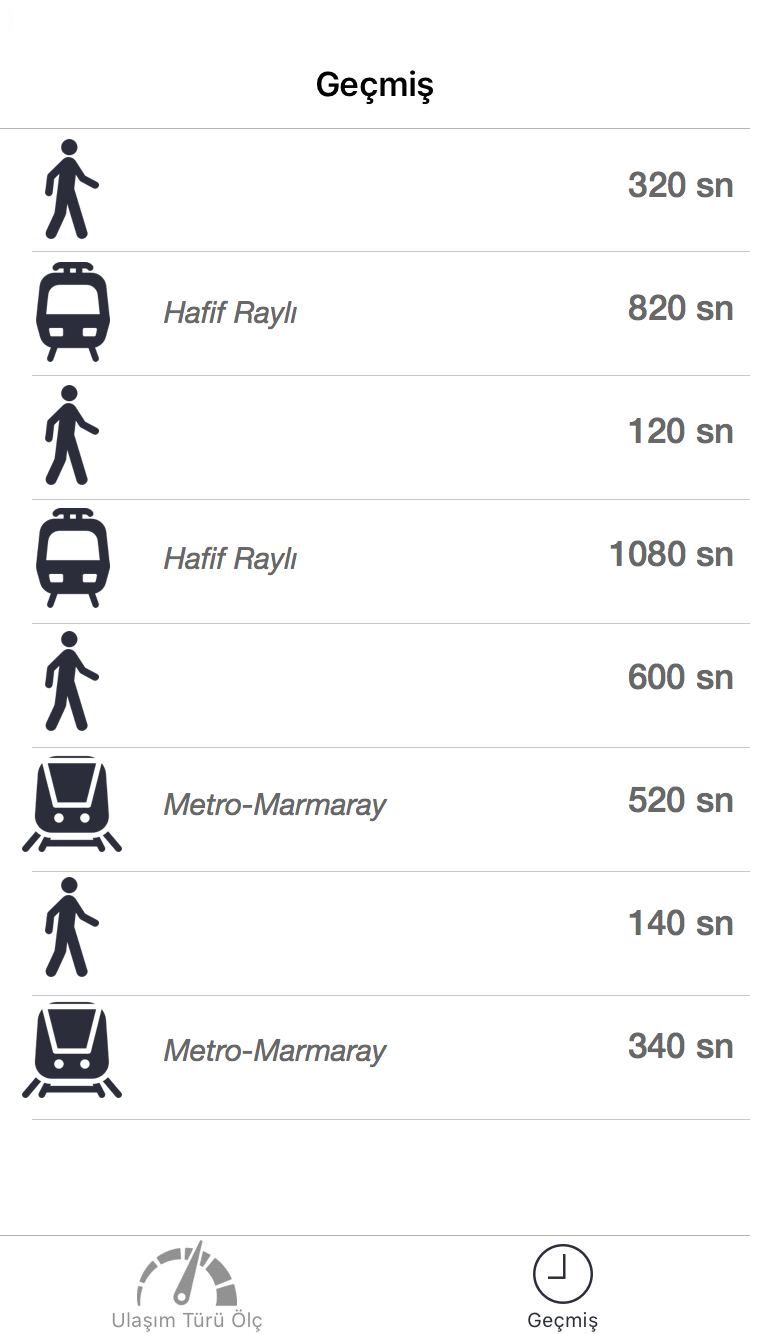
\includegraphics[scale=0.3]{projectChapters/images/rota_1.png}
\caption{2. güzergaha ait uygulama ekran çıktısı}
\end{figure}





%Tablo 7.1'de belirtilen 1. güzergaha ait uygulama ekran çıktısı Şekil 7.1'deki gibidir. 
%Sonuçlar incelendiğinde uygulama hafif raylı sınıfını metro-marmaray sınıfı ile karıştırmaktadır. Yürüme, tramvay ve araba sınıfları başarılı bir şekilde ayırt edilmektedir.


%Tablo 7.2'de belirtilen 2. güzergaha ait uygulama ekran çıktısı Şekil 7.2'deki gibidir. Uygulama otobüs-metrobüs sınıfını hafif raylı sınıfı ile karıştırmaktadır. Yürüme, metro-marmaray sınıfları başarılı bir şekilde ayırt edilmektedir.
